\section{二体問題$^\ast$ \label{ss:twobody}}

惑星と恒星の運動と軌道を考える。まず惑星と恒星をそれぞれ質点と考え(質量$m_1$,$m_2$、座標${\boldsymbol{r_1}},{\boldsymbol{ r_2}}$)、惑星と恒星の間に働く力を重力だけと考えることで、二体問題となり解析的に解くことができる。図\ref{fig:zahyou}のように${\boldsymbol{ r}} \equiv {\boldsymbol{r_2}} - {\boldsymbol{ r_1}}$とおく。軌道面上の円座標系${\bf e}_r=(\cos{\theta}, \sin{\theta})^\top$と${\bf e}_\theta=(-\sin{\theta}, \cos{\theta})^\top$で考える。${\bf r} = r {\bf e}_r$であり、また$\dot{{\bf e}}_r=\dot{\theta} (-\sin{\theta}, \cos{\theta})^T = \dot{\theta} \, {\bf e}_\theta $と$\dot{{\bf e}}_\theta=\dot{\theta}(-\cos{\theta}, -\sin{\theta})^T = - \dot{\theta} \, \dot{{\bf e}}_r$を用いると、
\begin{align}
\label{eq:speconv1}
\dot{\bf r} = \frac{d}{dt}{r {\bf e}_r} = \dot{r} {\bf e}_r + r \dot{{\bf e}}_r =  \dot{r} {\bf e}_r + r \dot{\theta} \, {\bf e}_\theta \\
\ddot{\bf r} = (\ddot{r} - r \dot{\theta}^2 ) {\bf e}_r + \left[ \frac{1}{r} \frac{d}{dt} (r^2 \dot{\theta} ) \right] \, {\bf e}_\theta
\end{align}
となる。重心を原点にとった時、$\boldsymbol{r_1}=-m_2/(m_1+m_2) \, \rv, \, \boldsymbol{r_2}= m_1/(m_1 + m_2) \,\rv$であるから、ラグランジアンは、換算質量$\mu = (m_1^{-1} + m_2^{-1})^{-1}$を用いて、
\begin{align}
L &= T - U = \frac{m_1}{2} |\dot{\boldsymbol{r_1}}|^2 + \frac{m_2}{2} |\dot{\boldsymbol{r_2}}|^2 + G \frac{m_1 m_2}{r} \nonumber \\
&= \frac{\mu}{2} [ \dot{r}^2 + (r \dot{\theta})^2 ] + G \frac{m_1 m_2}{r}
\end{align}
となる。

\begin{figure}[]
 \begin{center}
	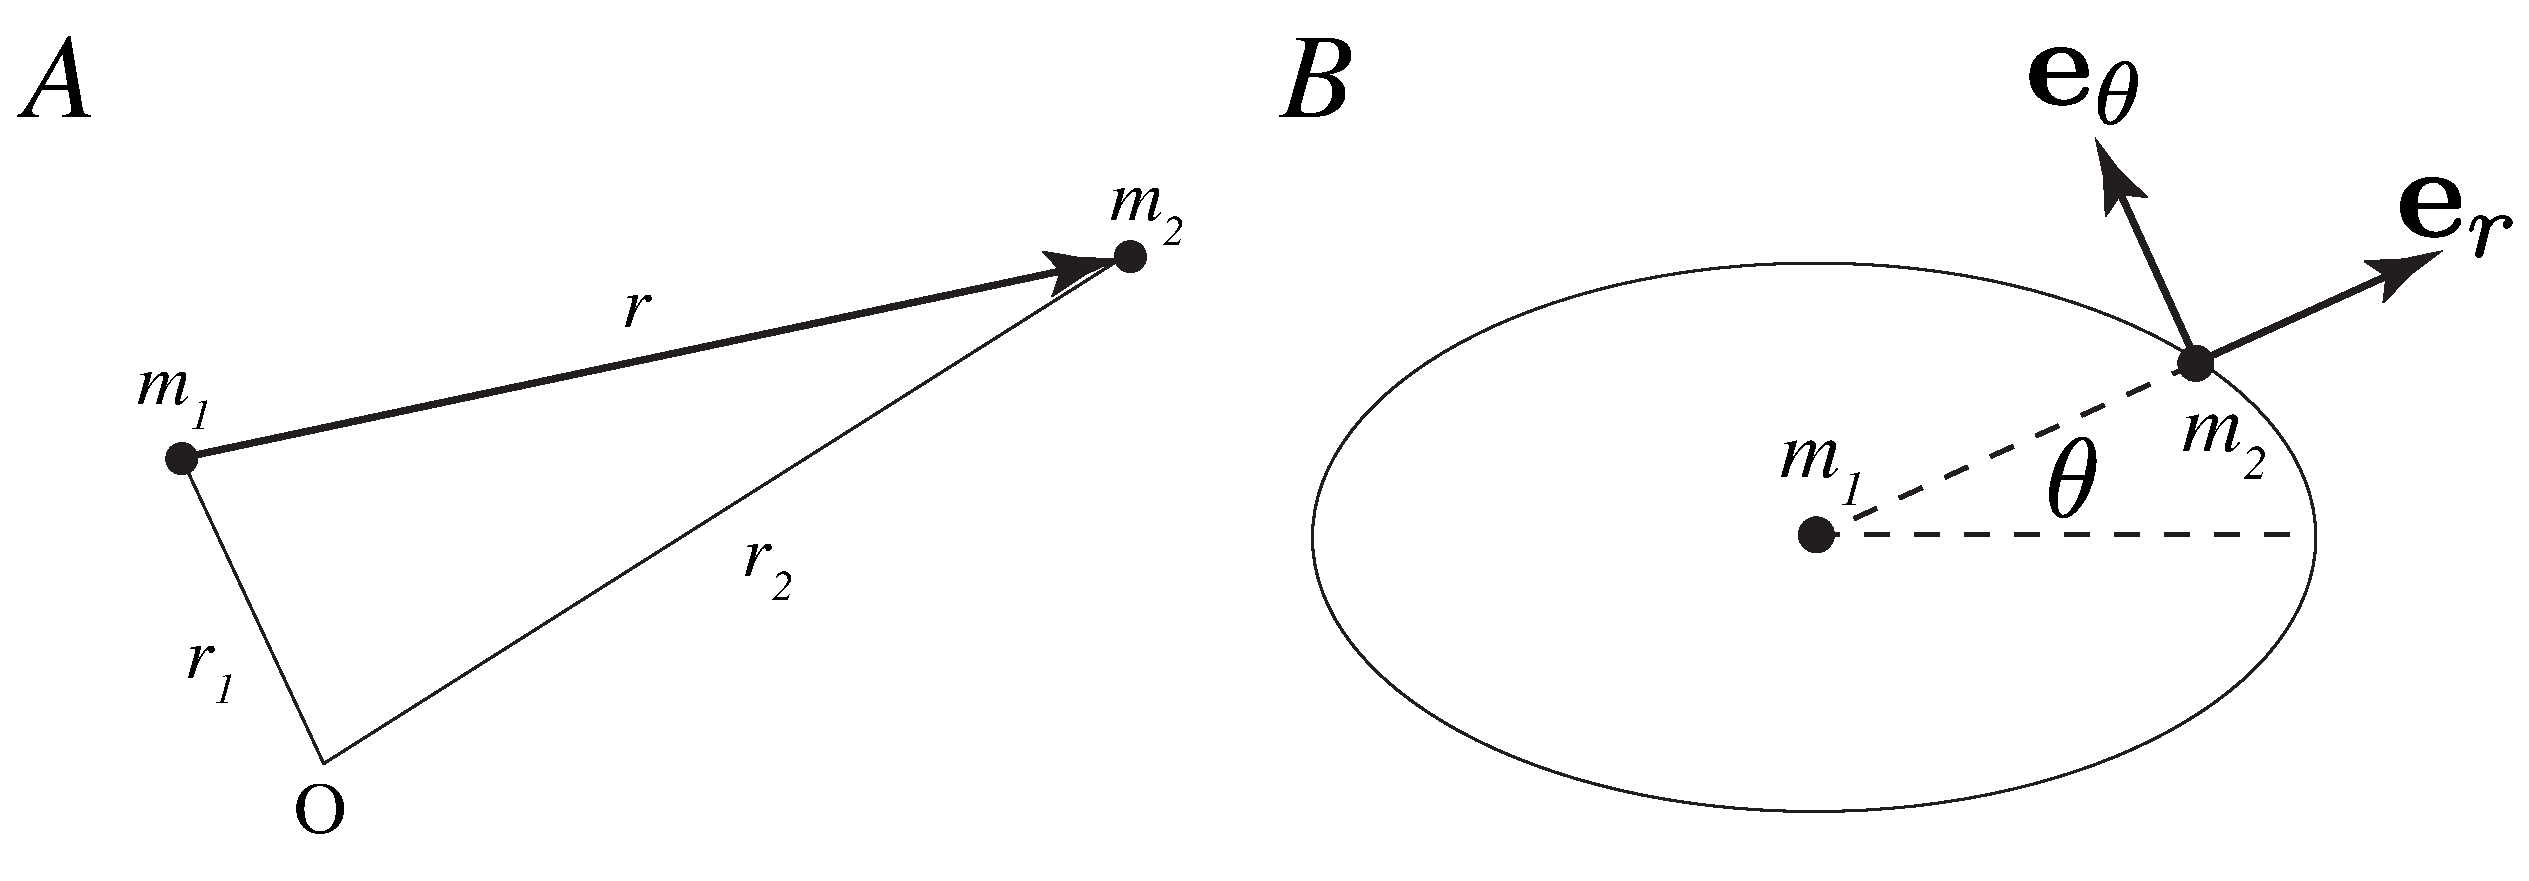
\includegraphics[width=\linewidth]{fig/zahyou.eps}
\end{center}
	\caption{座標系}
	\label{fig:zahyou}
\end{figure} 


\color{red}
\begin{itembox}{問題}
\footnotesize
\color{gray}
ラグランジュ方程式
\begin{align}
\frac{d}{dt} \left( \frac{\partial L}{\partial \dot{r}}\right) - \frac{\partial L}{\partial r} = 0, \,\,\,
\frac{d}{dt} \left( \frac{\partial L}{\partial \dot{\theta}}\right) - \frac{\partial L}{\partial \theta} &= 0
\end{align}
から

\begin{align}
\label{eq:eqrad}
 \ddot{r} - r \dot{\theta}^2 = - \frac{G (m_1+m_2)}{r^2}
\end{align}
と
$
\dot{\bf h} =  0
$
が得られることを確かめよ。ただし
$
{\bf h} \equiv {\bf r} \times \dot{\bf r} 
$
は軌道角運動ベクトルである。

すなわち軌道角運動量ベクトル${\bf h}$は、二体問題上は保存量である。これは質点が${\bf h}$に直交する平面(軌道面\index{きどうめん@軌道面})上の運動に制約されていることを意味する。
\end{itembox}
\color{black}



式(\ref{eq:eqrad})を変数変換し、$u \equiv 1/r$とする。$h u^2 = \dot{\theta}$、$\dfrac{d r}{d t} = \dfrac{d r}{d \theta} h u^2 = - h \dfrac{d u}{d \theta}$を用いて、
\begin{align}
\frac{d^2 u}{d \theta^2} + u = \frac{G (m_1 + m_2)}{h^2}
\end{align}
となる。これは非斉次二階微分方程式であり、斉次解は
\begin{align}
u_h = c_1 \cos{\theta} + c_2 \sin{\theta} = C_1 \cos{(\theta - C_2)}
\end{align}
のように書くことができる。非斉次解は明らかに
\begin{align}
u_i = \frac{G (m_1 + m_2)}{h^2}
\end{align}
であり、これらを足しあわせたものが一般解である。$G (m_1 + m_2)/h^2$をくくり出し、積分定数項を$e$, $\omega$とした一般解は
\begin{align}
u = \frac{G (m_1 + m_2)}{h^2} [ 1 + e \cos{(\theta - \omega)}]
\end{align}
とかける。$r=1/u$に戻すと、
\begin{align}
\label{eq:eqkep}
r =  \frac{h^2}{G (m_1 + m_2)} \frac{1}{ 1 + e \cos{(\theta - \omega)}} 
\end{align}

ところで、図\ref{fig:ellip}のような楕円を考えてみよう。楕円なので
\begin{align}
\label{eq:rellp}
r + r^\prime = 2 a
\end{align}
が成り立つ。また座標から
\begin{align}
\label{eq:rellp2}
(r^\prime)^2 &= (x_p + 2 e a )^2 + y_p^2 \nonumber \\
&= (r \cos{\theta} + 2 e a )^2 + (r \sin{\theta})^2
\end{align}
となる。式(\ref{eq:rellp},\ref{eq:rellp2})から$r^\prime$を消去すると、楕円のconic 方程式
\begin{align}
\label{eq:conic_orig}
r =  \frac{a (1-e^2)}{ 1 + e \cos{\theta}} 
\end{align}
が得られる。

\begin{figure}[]
 \begin{center}
	\includegraphics[bb=0 0 695 428,width=1.0\linewidth]{fig/ellip.png}
% \includegraphics[bb=0 0 474 461,width=1.0\linewidth]{fig/orbele.png}
\end{center}
	\caption{楕円}
	\label{fig:ellip}
\end{figure} 

長半径$a$、短半径$b$、またtrue anomary $f$を
\begin{align}
\label{eq:defkeppar1}
\frac{h^2}{G (m_1 + m_2)} &= a (1 - e^2) \\
\label{eq:defkeppar2}
b^2 &= a^2 (1 - e^2) \\
\label{eq:defkeppar3}
f &\equiv \theta - \omega  
\end{align}
と定義すれば、式(\ref{eq:eqkep})はconic方程式の形
\begin{align}
\label{eq:conic_kepler}
r =  \frac{a (1-e^2)}{ 1 + e \cos{f}} 
\end{align}
になることから、2体問題の解が楕円になることが確認される(ただし$0 \le e < 1$とする)。またtrue anomaly $f$は、periastron(近日点の太陽を恒星に変えたもの)から測った恒星惑星の角度に対応することが分かる。$\omega$はthe argument of periastronと呼ばれる量でconic方程式(\ref{eq:conic_orig})で表される楕円を半時計回りに$\omega$回転したということを表している。

ところで$\dot{A}$は一定であるから楕円面積
\begin{align}
A = \pi a b = \frac{h}{2} P
\end{align}
とかける。ここに$P$は公転周期である。これを変形すると
\begin{align}
\label{eq:kep3}
 P^2 = \frac{4 \pi^2}{G (m_1+m_2)} a^3 
\end{align}
となる。公転周期の自乗は質量に反比例、軌道長半径の3乗に比例することが分かる(ケプラーの第三法則)。円軌道の場合、公転角速度は$1/\sqrt{G (m_1+m_2) a}$であることも分かる。式(\ref{eq:defkeppar1})を用いて$G$を消すことで角運動量表記
\begin{align}
\label{eq:kep3_1}
 P = \frac{2 \pi a^2 \sqrt{1-e^2}}{h} 
\end{align}
もえられる。

\begin{figure}[]
 \begin{center}
%	\includegraphics[bb=0 0 695 428,width=1.0\linewidth]{fig/ellip.png}
 \includegraphics[bb=0 0 474 461,width=1.0\linewidth]{fig/orbele.png}
\end{center}
	\caption{座標系}
	\label{fig:ellip}
\end{figure} 

平均運動は
\begin{align}
    n \equiv \frac{2 \pi}{P}
\end{align}
で定義される。式(\ref{eq:kep3_1})を用いることで
\begin{align}
\label{eq:mean_motion}
    n = \frac{h}{a^2 \sqrt{1-e^2}}
\end{align}
とも表せる。

\section{三次元空間における二体問題 \label{ss:threedtwobody}}

前章では、二次元平面上での二体運動を考えた。実際の天体は観測者から見て三次元空間上に存在しているので、軌道を3次元回転する必要がある。
観測者からみた傾きである軌道傾斜角(orbital inclination)を$i$で、azimuth方向の定義をlongitude of ascending node $\Omega$で指定する。これら$a,e,\omega, f, i, \Omega$の六つのパラメタを指定すれば、三次元空間における二体問題の軌道が一意に決定される。

これらの回転を回転行列で表してみよう。まず、元となる楕円はconic方程式(\ref{eq:conic_orig})であらわされる図\ref{fig:ellip}のものとしよう。$z$軸を紙面に垂直にとるとする。
\begin{itemize}
\item (1) conic方程式(\ref{eq:conic_orig})を$z$軸周りに反時計回りに$\omega$回したものが二体問題の楕円の方程式(\ref{eq:conic_kepler})であった。
\item (2) 次に$x$軸周りに反時計方向に$i$回すと軌道面が天球に対して$i$傾く事になる。\\
\item (3) 最後に$z$軸周りに$\Omega$、つまり天球のazimuth方向の回転の自由度が残る。
\end{itemize}

これらの回転行列を順に楕円を表す$\rv = (r \cos{\theta}, r \sin{\theta},0)$に対してかける。まず(1)は
% ---- 1. position in the orbital plane ---------------------------------
\begin{align}
\rv &=
\begin{pmatrix}
r\cos\theta\\
r\sin\theta\\
0
\end{pmatrix}
=
\begin{pmatrix}
r\cos\!\bigl(f+\omega\bigr)\\
r\sin\!\bigl(f+\omega\bigr)\\
0
\end{pmatrix}
\end{align}
である。次に(2)は
% ---- 2. rotation by the inclination i (about the x-axis) --------------
\begin{align}
\rv^\prime &=
\begin{pmatrix}
1 & 0        & 0\\
0 & \cos i   & -\sin i\\
0 & \sin i   &  \cos i
\end{pmatrix}
\rv \\
&=
\begin{pmatrix}
r\cos\!\bigl(f+\omega\bigr)\\
r\sin\!\bigl(f+\omega\bigr)\cos i\\
r\sin\!\bigl(f+\omega\bigr)\sin i
\end{pmatrix}
\end{align}
となる。
% ---- 3. rotation by the longitude of ascending node Ω (about the z-axis)
最後に(3)は
\begin{align}
\rv^{\prime\prime} &=
\begin{pmatrix}
\cos\Omega & -\sin\Omega & 0\\
\sin\Omega &  \cos\Omega & 0\\
0          &  0          & 1
\end{pmatrix}
\rv^\prime \\
&=
\begin{pmatrix}
r\cos\!\bigl(f+\omega\bigr)\cos\Omega
 - r\sin\!\bigl(f+\omega\bigr)\cos i\,\sin\Omega\\[4pt]
r\cos\!\bigl(f+\omega\bigr)\sin\Omega
 + r\sin\!\bigl(f+\omega\bigr)\cos i\,\cos\Omega\\[4pt]
r\sin\!\bigl(f+\omega\bigr)\sin i
\end{pmatrix}
\\
\label{eq:threed}
&\equiv
\begin{pmatrix}
X\\[2pt] Y\\[2pt] Z
\end{pmatrix}.
\end{align}
となり、三次元空間での軌道$(X,Y,Z)$が得られた。

\section{二体問題を時間について求める}
二体問題の解はtrue anomaly $f$の関数、つまり$r = r(f)$として書かれていた。しかし現実の観測では、二体問題はなんであれ時間の関数として観測される。そこで時間表記$r = r(t)$をどのように求めるか考えてみよう。

方針は以下のとおりである。まず
\begin{align}
        v^2 &= \dot{\rv} \cdot \dot{\rv} 
        = (\dot{r} {\ev}_r + r \dot{f} {\ev}_\theta) \cdot (\dot{r} {\ev}_r + r \dot{f} {\ev}_\theta) \nonumber \\
        \label{eq:v2_1}
        &= \dot{r}^2 + r^2 \dot{f}^2 \\
        \label{eq:v2_2}
        &=  \dot{r}^2 + \frac{h^2}{r^2} 
\end{align}
を考える($h = r^2 \dot{f}$を用いた)。そして、
\begin{itemize}
    \item (1) $v^2$を式(\ref{eq:v2_2})から$r$,$\dot{r}$を$f$の関数に変換し$v^2 (f)$で表す
    \item (2) $v^2(f)$をConic方程式で$v^2(r)$に変換
    \item (3) $v^2 = \dot{r}^2 + h^2/r^2$と等置して$r, \dot{r}$の式、つまり$r$の時間に関する微分方程式を得る
\end{itemize}

(1)について$r$から$f$への変換はConic方程式(\ref{eq:conic_kepler})を用いればよい。また$\dot{r}$を$f$に変換するには
\begin{align}
\label{eq:dotr}
\dot{r} &= \frac{h}{a(1-e^{2})}\,e\sin f 
\end{align}
を用いる。

\begin{itembox}{$\clubsuit$式(\ref{eq:dotr})の導出}
\footnotesize
\color{gray}
\begin{align}
    \dot r
  &=\frac{df}{dt}
   \,\frac{d}{df}\!
     \left(
       \frac{a(1-e^{2})}{1+e\cos f}
     \right)
  =\dot f\,
    \frac{a(1-e^{2})\,e\sin f}{\bigl(1+e\cos f\bigr)^{2}}
    \nonumber \\
    &= \dot{f} \frac{a (1-e^2)}{1 + e \cos{f}} \frac{e \sin{f}}{1 + e \cos{f}} = r \dot{f} \frac{e \sin{f}}{1 + e \cos{f}} \nonumber\\
&= \frac{h}{r} \frac{e \sin{f}}{1 + e \cos{f}}
= \frac{h}{a(1-e^{2})}\,e\sin f
\end{align}
\end{itembox}

つまり
\begin{align}
    v^2 &= \dot{r}^2 + (r \dot{f})^2 = \dot{r}^2 + \frac{h^2}{r^2} \nonumber \\
    &= \frac{h^2}{a^2(1-e^2)^2} [2 (1 + e\cos{f}) + e^2 - 1 ] = v^2(f)
\end{align}



次に$v^2(f)$を再度Conic方程式を用いて$r$の関数に変換する(2)の手順は、
\begin{align}
    v^2(r) &= \frac{h^2}{a (1 - e^2)} \left( \frac{2}{r} - \frac{1}{a} \right)
\end{align}
となる。(3)より$r$の時間微分方程式
\begin{align}
\label{eq:rde}
    \dot{r}^2 - \frac{h^2}{a (1-e^2)}  \left( \frac{2}{r} - \frac{1}{a} \right) + \frac{h^2}{r^2} = 0
\end{align}
を得る。この方程式はそのまま解くことはできない。そこでeccentric anomaly $E$を導入する。
\begin{align}
\label{eq:eanomaly}
    r = a (1 - e \cos{E})
\end{align}
この$E$を用いて、微分方程式(\ref{eq:rde})を$E$, $\dot{E}$の微分方程式に変換すると
\begin{align}
\label{eq:dee}
    \dot{E} = \frac{n}{1 - e \cos{E}}
\end{align}
また、天下りであるが、この解は
\begin{align}
    E - e \sin{E} = n (t -t_0)
\end{align}
で与えられる(微分することで式(\ref{eq:dee})が成り立つことを確かめよ)。ここで時間変数の代理としてMean anomaly $M$を
\begin{align}
    M \equiv n (t - t_0)
\end{align}
と定義することにより
\begin{align}
\label{eq:dee_sol_M}
    f(E) = E - e \sin{E} - M = 0
\end{align}
を解くことで$E$が求まる。

\begin{itembox}{$\clubsuit$式(\ref{eq:dee})の導出}
\footnotesize
\color{gray}
\begin{align}
  \frac{2}{r}-\frac{1}{a}
    &=\frac{1}{a}\!\left(\frac{2}{1-e\cos E}-1\right)     \nonumber \\
    &=\frac{1}{a}\,\frac{1+e\cos E}{1-e\cos E}
      \;=\;
      \frac{1}{a}\,
      \frac{1-e^{2}\cos^{2}E}{(1-e\cos E)^{2}}\;.
\end{align}

\begin{align}
 &\frac{h^{2}}{r^{2}}
 -\frac{h^{2}}{a^{2}(1-e^{2})}\!
  \left(\frac{2}{r}-\frac{1}{a}\right) \nonumber \\
 &= \frac{h^{2}}{a^{2}(1-e\cos E)^{2}}
    -\frac{h^{2}(1-e^{2})}{a^{2}(1-e\cos E)^{2}(1-e^{2})} \nonumber \\
 &=\frac{h^{2}(1-e^{2})}{a^{2}(1-e\cos E)^{2}(1-e^{2})} -\frac{h^{2}(1-e^{2}\cos^{2}E)}{a^{2}(1-e\cos E)^{2}(1-e^{2})}\nonumber \\
 &= -\frac{h^{2}e^{2}\bigl(1-\cos^{2}E\bigr)}
        {a^{2}(1-e\cos E)^{2}(1-e^{2})}
\end{align}

\begin{align}
     \dot r &=\frac{dE}{dt}\,
         \frac{d}{dE}\bigl(a(1-e\cos E)\bigr)
     =\dot E\,a e\sin E \\
  \dot r^{2}
    &=\dot E^{2}\,a^{2}e^{2}\sin^{2}E
\end{align}
これらの式より、
\begin{align}
    \dot E^{2}\,a^{2}e^{2}\bigl(1-\cos^{2}E\bigr)
  =
  \frac{h^{2}\,e^{2}\bigl(1-\cos^{2}E\bigr)}
       {a^{2}(1-e\cos E)^{2}(1-e^{2})}
\end{align}
つまり
\begin{align}
    \dot E^{2}
   =\frac{h^{2}}
          {a^{4}(1-e\cos E)^{2}(1-e^{2})}
\end{align}
$\dot{E} > 0$に軸を取るとすると、
\begin{align}
    \dot E
 &=\frac{h}{a^{2}\sqrt{1-e^{2}}\,(1-e\cos E)} \\
 & = \frac{n}{1 - e \cos{E}}
\end{align}
を得た。最後の変形は平均運動(\ref{eq:mean_motion})を用いた。
\end{itembox}

また$E$と$f$の関係は式(\ref{eq:eanomaly})と二体問題の円錐方程式(\ref{eq:conic_kepler})から
\begin{align}
\label{eq:Efrel}
\cos{f} = \frac{\cos{E} - e}{1 - e \cos{E}}
\end{align}

これにより、周期$P$とオフセット$t_0$が分かれば時間$t$からmean anomaly $M$か計算でき、数値計算で式(\ref{eq:dee_sol_M})を解くことで$E$が、さらに式(\ref{eq:Efrel})からtrue anomaly $f$を求めることができる。\\

\subsubsection{Newton-Raphson法により式(\ref{eq:dee_sol_M})を解く}

非線形方程式$f(E)=0$は数値的に求めることが必要である。このための方法の一つとしてNewton-Raphson法を紹介する。Newton-Raphson法は図\ref{fig:newton_raphson}にしめすように、まず初期値$E_1$から初めて、$f(E_1)$に接する直線を求め、その直線と原点との交点を解析的に求め$E_2$とする。この手続きを$n$回繰り返すという手順である。$i$番目の手続きでは接線(つまり$f(E)$を$E_i$でテイラー展開した一次の項までの近似式)は
\begin{align}
\label{eq:nrm}
   y = f(E_i) + f^\prime(E_i) (E - E_i) 
\end{align}
となることから
\begin{align}
\label{eq:update_newton}
    E_{i+1} &= E_i + \Delta E_i \\
    \Delta E_i &\equiv - \frac{f(E_i)}{f^\prime(E_i)}
\end{align}
となる。$\Delta E_i$を$i$番目の更新項(update term)とよぶ\footnote{単に$f(E)$をテイラー展開して1次まで残した近似を用いて解を更新していくとみることもできる。すなわち
\begin{align}
\label{eq:nrm_f}
   f(E) \approx f(E_i) + f^\prime(E_i) (E - E_i) = 0
\end{align}
の解を$E_{i+1}$として、繰りかえすことに対応している。}。この手続きを収束条件の判定値を$\epsilon$として$ |E_{i+1} - E_{i}| < \epsilon$となるまで繰り返し、条件を満たした$E_i$を近似解とすればよい。

式(\ref{eq:nrm})の計算には$f$の微分が必要である。式(\ref{eq:dee_sol_M})より
\begin{align}
    f^\prime(E) = 1 - e \cos{E}
\end{align}
である。

\begin{figure}[]
 \begin{center}
 \includegraphics[width=1.0\linewidth]{fig/newton_raphthon.png}
\end{center}
	\caption{Newton-Raphson法の概念図。}
	\label{fig:newton_raphson}
\end{figure} 

\begin{itembox}{二次最適化としてのNewton法$^\dagger$}
\footnotesize
\color{gray}
コスト関数$Q(x)$を最小にする$x=x^\ast$を求める最適化問題
\begin{equation}
   x^\ast = \mathrm{minimize}_{x} \,\, Q(x)  
\end{equation}
の解法として、停留点条件
$d Q(x)/d x = 0$
をNewton-Raphson法で求めることができる。この場合、
$f (x) = Q^\prime (x)$
として、式(\ref{eq:update_newton})を用いると、更新式は
\begin{align}
x_{i+1} &= x_i + \Delta x_i \\ 
\Delta x_i &\equiv - \frac{Q^\prime (x_i)}{Q^{\prime\prime}(x_i)}  
\end{align}
となり、$Q(x)$の二回微分が必要であることから、二次の最適化と呼ばれる。ちなみに最適化の文脈ではRaphsonが省略され、単にNewton法と呼ばれることが多い。

一般に多次元のNewton法も同様に構成できる。多次元のテイラー展開より
\begin{align}
\fv(\xv) \approx \fv(\xv_i) + \Jv (\xv_i) (\xv - \xv_i) = \boldsymbol{0}
\end{align}
をみたす$\xv$が次の更新点となるので、
\begin{align}
    \xv_{i+1} &= \xv_{i} + \Delta \xv_i \\
    \label{eq:second_newton}
    \Delta \xv_i &\equiv - \Jv^{-1} (\xv_i) \fv(\xv_i)
\end{align}
となる。ただし$\Jv (\xv_i)$はヤコビアンである。
\end{itembox}


